%!Tex Root = ../main.tex
% ./Packete.tex
% ./Design.tex
% ./Deklarationen.tex
% ./Vorbereitung.tex
% ./Aufgabe1.tex
% ./Aufgabe3.tex
% ./Aufgabe4.tex
% ./Appendix.tex

\section{Aufgabe 2}

\setcounter{exercise}{1}

\begin{frame}[fragile, allowframebreaks]{Aufgabe \thesection}{RETI}
    \begin{requirementsnoinc}
      \begin{itemize}
        \item Seien $a, b\in \mathrm{N}$. Wenn wir wiederholt den \alert{Euklidischer Algorithmus} durchführen:
        \begin{align*}
          a &= b\cdot q_1 + r_1\\
          b &= r_1\cdot q_2 + r_2\\
          r_1 &= r_2\cdot q_3 + r_3\\
              &\ldots\\
          r_{n-3} &= r_{n-2}\cdot q_{n-1} + r_{n-1}\\
          r_{n-2} &= r_{n-1}\cdot q_{n} + 0
        \end{align*}
        dann gilt: $r_{n-1} = ggt(a, b)$.
        \item $g g t(a,b)=g g t(m a x(a,b)-m i n(a,b),m i n(a,b)){\mathrm{~und~}}g g t(a,0)=a$
      \end{itemize}
    \end{requirementsnoinc}  
    \begin{requirementsnoinc}
      \begin{itemize}
        \item \alert{Beweis:} \url{https://www.youtube.com/watch?v=8cikffEcyPI}
        \begin{itemize}
          \item \alert{Anmerkung zum Beweis im Video:} Wann immer wir eine geordnete Folge von Zahlen haben, deren Wert immer kleiner wird und nichtnegativ sind, können wir sicher sein, dass diese Folge den Wert $0$ erreicht.
          \item \alert{Man braucht folgende Definition für GGT:} Eine Zahl $g$ wird \enquote{größter gemeinsamer Teiler} von $a$ und $b$ genannt, wenn sie die folgenden beiden Bedingungen erfüllt:
          \begin{enumerate}
            \item $g$ is a \enquote{gemeinsamer Teiler} von $a$ und $b$. In anderen Worten: $g$ teilt $a$ und $g$ teilt $b$
            \item Wenn $d$ ein gemeinsamer Teiler von $a$ und $b$ ist dann: $d$ teilt $g$
          \end{enumerate}
        \end{itemize}
        \item Wichtig für RSA, da \alert{Primfaktorzerlegung} mit der man den GGT zweier Zahlen berechnen kann \alert{sehr langsam} ist, aber der \alert{Euklidische Algorithmus} den GGT zweier Zahlen \alert{sehr schnell} berechnen kann ohne die beiden Zahlen vollständig faktorisieren zu müssen.
        % https://youtu.be/8cikffEcyPI
      \end{itemize}
    \end{requirementsnoinc}  
    \begin{requirementsnoinc}
      \begin{itemize}
        \item \alert{Was eigentlich gerechnet wird:} Division mit Rest
    \begin{transformation}[0.4][0.2][0.4]
      $\textcolor{PrimaryColor}{a} = \textcolor{SecondaryColor}{b}\cdot \textcolor{gray}{q_1} + \textcolor{PrimaryColorDimmed}{r_1}$
      \arrowx{eigentlich}
      $\displaystyle\frac{\textcolor{PrimaryColor}{a}}{\textcolor{SecondaryColor}{b}} = \textcolor{gray}{q} \textcolor{PrimaryColorDimmed}{\text{ Rest } r}$
    \end{transformation}
        \item \alert{Algorithmus vereinfacht ausgedrückt:}
        \begin{enumerate}
          \item \textcolor{SecondaryColor}{Divisor} nach \textcolor{PrimaryColor}{vorne}
          \item \textcolor{PrimaryColorDimmed}{Rest} zum \textcolor{SecondaryColor}{Divisor}
          \item den \textcolor{gray}{Qutoienten} ignorieren
        \end{enumerate}
        \item Euklidischer Algorithmus am Beispiel $a=12$ und $b=16$:
          \begin{align*}
            \textcolor{PrimaryColor}{12} &= \textcolor{SecondaryColor}{16}\cdot \textcolor{gray}{0} + \textcolor{PrimaryColorDimmed}{12}\\
            \textcolor{SecondaryColor}{16} &= \textcolor{PrimaryColorDimmed}{12}\cdot \textcolor{gray}{1} + \boxed{4}\\
            \textcolor{PrimaryColorDimmed}{12} &= \boxed{4}\cdot \textcolor{gray}{3} + 0\\
          \end{align*}
          dann gilt: $4 = ggt(12, 16)$.
      \end{itemize}
    \end{requirementsnoinc}
    \begin{solutionnoinc}
        \begin{linenums}
            \numberedcodebox[minted language=py, minted options={}] {./figures/gcd.py}
        \end{linenums}
        \begin{itemize}
          \item \alert{letzter Durchlauf:} $\boxed{4} = 0\cdot \textcolor{gray}{whatever} + 4$
        \end{itemize}
    \end{solutionnoinc}
    \begin{solutionnoinc}
        \begin{linenums}
            \numberedcodebox[minted language=c, minted options={}] {./figures/gcd.picoc}
        \end{linenums}
    \end{solutionnoinc}
    \begin{solutionnoinc}
        \begin{itemize}
          \item Modulo ist $q$ Mal die eine Zahl von der anderen abziehen: $a = b \cdot q + r$. Für den GGT muss das Modulo nehmen wie aus der Funktion $gcd$ bekannt fortgeführt werden. Bei genauer Betrachtung lässt sich das gesamte Vorgehen auf folgende Fälle beschränken:
            \begin{equation*}
              \begin{dcases*}
                b = b-a & if $a<b$\,, \\[0.1cm]
                a = a-b & if $a>b$\,, \\[0.1cm]
                a \text{ oder } b & if $a=b$\,.
              \end{dcases*}
            \end{equation*}
            bis: $a = b$
          \item damit am Ende der Rest $0$ sein kann, muss es am Ende der Fall sein, dass $x - y$ gerechnet wird und $x=y$ ist, da nur so $0$ als Rest rauskommen kann
        \end{itemize}
    \end{solutionnoinc}
    \begin{solutionnoinc}
        \begin{itemize}
          \item \alert{Beispiel:}
            \begin{align*}
              \textcolor{PrimaryColor}{20} &= \textcolor{PrimaryColor}{32} - \textcolor{SecondaryColor}{12}\\
              \textcolor{PrimaryColor}{8} &= \textcolor{PrimaryColor}{20} - \textcolor{SecondaryColor}{12}\\
              \textcolor{PrimaryColor}{4} &= \textcolor{SecondaryColor}{12} - \textcolor{PrimaryColor}{8}\\
              \boxed{\textcolor{PrimaryColor}{4}} &= \textcolor{SecondaryColor}{8} - \boxed{\textcolor{PrimaryColor}{4}}\\
            \end{align*}
        \end{itemize}
    \end{solutionnoinc}
    \begin{solutionnoinc}
        \centering
        \resizebox{\textwidth}{!}{
            \begin{minipage}[t]{18cm}
                \begin{linenums}
                    \numberedcodebox[minted language=text, minted options={}]{./figures/gcd_sol.reti}
                \end{linenums}
            \end{minipage}
        }
    \end{solutionnoinc}
    \begin{solutionnoinc}
        \centering
        \href{https://asciinema.org/a/586086}{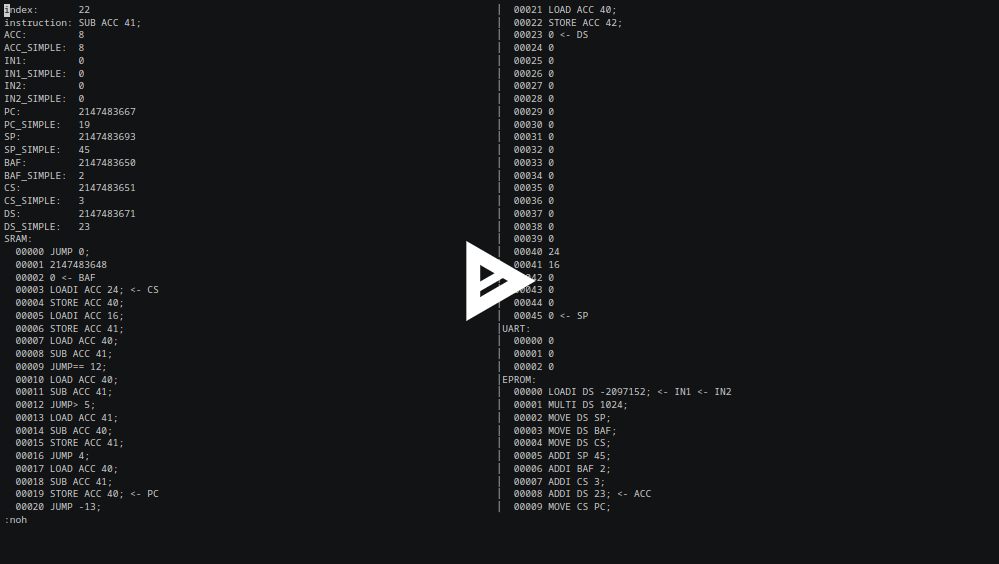
\includegraphics[width=0.6\textwidth]{./figures/gcd_sol_play.png}}
    \end{solutionnoinc}
\end{frame}
